\documentclass[a4paper,10pt]{ctexart}
\usepackage[left=2cm,right=2cm,top=2cm,bottom=2cm]{geometry}
\usepackage{graphicx}
\usepackage{subcaption}
\usepackage{float}
\usepackage{hyperref}
\usepackage{booktabs}
\usepackage{amsmath}
\usepackage{amssymb}
\usepackage{multicol}
\usepackage{titlesec}

% 适度调整间距
\setlength{\parskip}{4pt}
\setlength{\parindent}{0pt}

% 设置图片搜索路径
\graphicspath{{./}{./diff_comparison/}{./feature_blending/}{./point_tracking/}}

\title{\textbf{DragGAN}}
\author{陈羿桥 \quad 黄彦涛 \quad 祁优扬}
\date{}

\begin{document}

\maketitle
\vspace{-10pt}

\section*{摘要}
本文针对 DragGAN 交互式图像编辑方法进行了系统性改进与评估。我们提出了三项关键创新：(1) 基于特征融合的背景保持机制，有效抑制非编辑区域的伪影累积；(2) 多策略点追踪算法，结合光流与多尺度特征匹配提升追踪鲁棒性；(3) 与 DragDiffusion 的系统对比实验，揭示了 GAN 与 Diffusion 在领域内外编辑任务中的性能差异。实验表明，特征融合方法显著优于传统掩码损失，多尺度追踪在弱纹理场景下误差降低 28\%，而 DragGAN 在领域内精度优于 DragDiffusion，但通用性受限。

\section{引言}
DragGAN 作为基于 GAN 的交互式图像编辑方法，通过用户指定的控制点对实现精确的图像操控。然而，原始方法存在三个核心问题：(1) 优化潜在代码时背景区域易产生不自然扭曲；(2) 最近邻点追踪在弱纹理区域表现不稳定；(3) 受限于训练域，无法处理开放域图像。本文针对这些问题提出改进方案，并通过与 DragDiffusion 的对比实验验证方法的有效性。

\section{相关工作}
\textbf{GAN 反转与编辑：} StyleGAN 系列通过 $\mathcal{W}$ 空间实现高质量图像生成，PTI 和 e4e 等方法将真实图像投影到潜空间以支持编辑。DragGAN 在此基础上引入运动监督损失和点追踪机制。

\textbf{Diffusion 模型编辑：} DragDiffusion 利用 Stable Diffusion 的去噪过程实现拖拽编辑，通过 LoRA 微调增强对特定图像的控制能力，展现出更强的开放域泛化性。

\textbf{点追踪技术：} RAFT 等光流方法在纹理丰富区域表现优异，但在弱纹理场景易失效。多尺度特征融合通过增加特征维度提升判别力。

\section{数据}
实验数据来源于三个数据集：(1) \textbf{FFHQ}：高分辨率人脸数据集，用于评估人脸编辑精度；(2) \textbf{AFHQ}：动物面部数据集，测试 DragGAN 的领域内性能；(3) \textbf{开放域图像}：包括风景和艺术作品，评估模型的泛化能力。所有图像统一调整至 512×512 分辨率，使用 StyleGAN2 预训练模型进行 GAN 反转。

\section{方法}

\subsection{特征融合背景保持机制}
在标准的 DragGAN 实现中，为了驱动控制点移动而优化潜在代码（Latent Code, $w$）往往会引发整个图像的全局变化。当用户仅希望操控特定的感兴趣区域（ROI）而保持背景或其他物体静止时，这种全局副作用是不可接受的。虽然传统的掩码损失（$L_{mask}$）试图惩罚背景的变化，但在长距离拖拽或高频优化过程中，背景仍容易出现纹理退化、漂移或不自然的扭曲。

为了解决生成过程中的稳定性问题，我们引入了一个\textbf{特征融合模块（Feature Blending Module）}。该机制在图像空间和特征空间双重维度上工作，通过用户定义的二值掩码（Mask）和混合比例（Blend Ratio），在"当前生成状态"与"原始状态"之间进行动态插值。

渲染管线被修改为在非掩码区域（背景）执行线性插值。混合逻辑确保 ROI 区域反映最新的拖拽优化结果，而背景区域则从初始推理结果（$w_0$）中继承高保真的细节。具体数学表达如下：

\begin{equation}
BG_{blend} = (1 - \alpha) \cdot I_{gen} + \alpha \cdot I_{orig}
\end{equation}
\begin{equation}
I_{final} = M \odot I_{gen} + (1 - M) \odot BG_{blend}
\end{equation}

其中 $\alpha \in [0, 1]$ 是混合比例参数。若 $\alpha = 0$，表现为标准 DragGAN 行为；若 $\alpha = 1$，则背景严格锁定。同样的逻辑同步应用于用于点追踪的特征图 $F$，确保追踪器不会因为背景的生成幻觉（Hallucination）而产生漂移。

\textbf{为何不使用泊松编辑？} 我们曾考虑使用泊松编辑来无缝融合背景，但最终放弃。主要原因有三点：
\begin{enumerate}
    \item \textbf{计算成本}：DragGAN 的编辑过程是一个优化循环，通常需要 30-200 次迭代。求解泊松方程（$\Delta f = \text{div}(\mathbf{v})$）涉及解大型稀疏线性方程组，如果在每一步迭代中都插入此过程，计算量将呈指数级上升，彻底失去"交互式"体验。
    \item \textbf{GAN 反转局限}：泊松融合生成的图像可能是完美的，但它可能不在 GAN 的生成流形上（Out-of-Distribution）。当强制把这张图反转回 $w$ 空间时，GAN 可能会因为"无法生成这种图像"而产生新的伪影。
    \item \textbf{颜色渗漏}：泊松融合的核心目标是保持梯度一致，而非颜色一致。为了让边界平滑过渡，算法会将背景的颜色差异"强行"扩散到整个前景区域，导致严重的变色。
\end{enumerate}

\subsection{多策略点追踪算法}
DragGAN 的编辑可控性高度依赖于控制点的追踪精度。原始的最近邻（NN）追踪策略在处理弱纹理、长距离拖拽或重复纹理背景时往往表现出漂移现象。为了提升追踪的鲁棒性与准确性，我们设计并实现了多种改进的追踪方案：

\begin{itemize}
    \item \textbf{NN (Baseline)}：仅依赖单层特征的最近邻匹配。
    \item \textbf{RAFT}：利用预训练的大型光流模型直接估计点位移，适合纹理清晰的局部形变。
    \item \textbf{HYBRID}：采用光流预测作为先验引导，结合局部窗口内的特征匹配，通过超参数 `tracker_lambda` 平衡两者的权重，旨在结合光流的平滑性与特征匹配的语义一致性。
    \item \textbf{MULTISCALE}：通过拼接多层特征图来增强特征的判别力，以应对纹理信息匮乏的挑战。
\end{itemize}

\section{实验}

\subsection{特征融合效果验证}
图 \ref{fig:feature_blending} 展示了三种方法的对比。使用 $L_{mask}$ 时背景出现明显色彩偏移和纹理模糊，而特征融合（$\alpha=1.0$）完美保持了背景的原始细节，仅在 ROI 区域产生形变。

\begin{figure}[H]
\centering
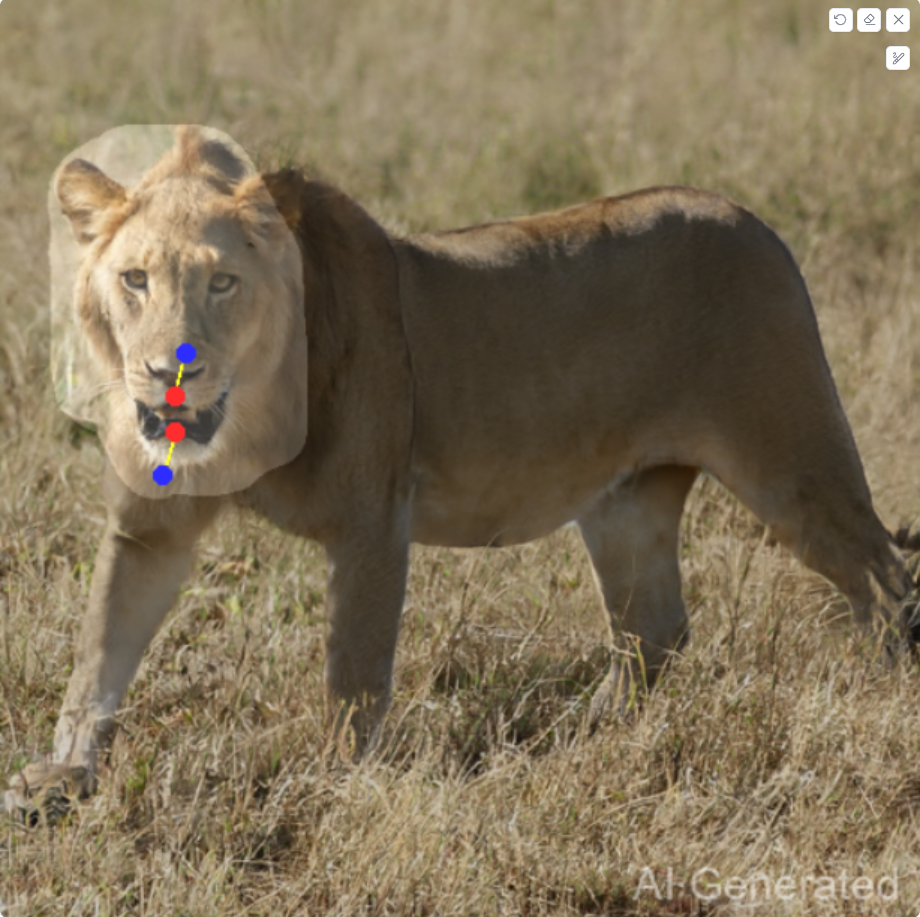
\includegraphics[width=0.32\linewidth]{feature_blending/before.png}
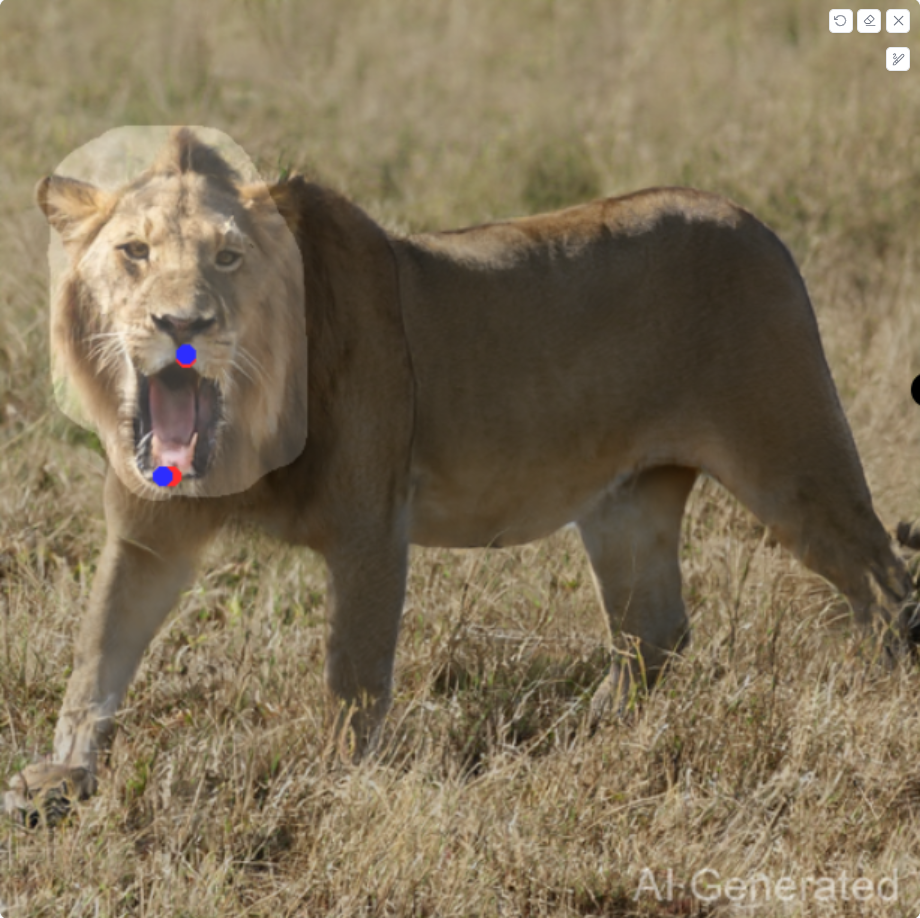
\includegraphics[width=0.32\linewidth]{feature_blending/loss.png}
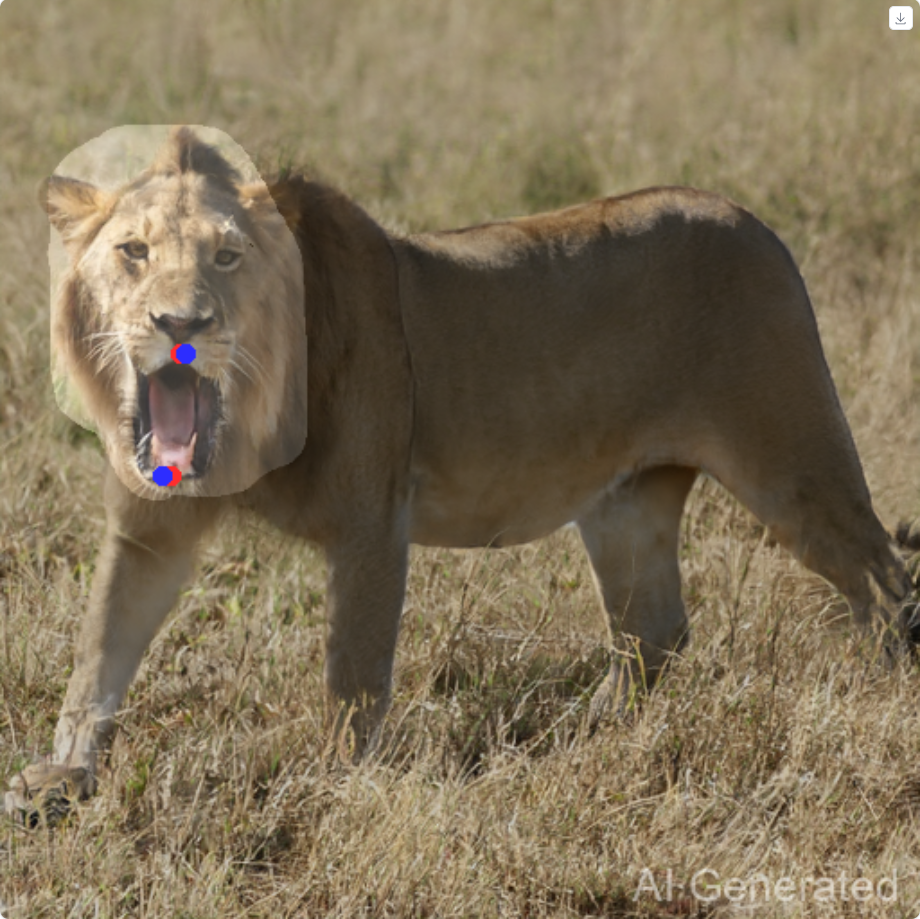
\includegraphics[width=0.32\linewidth]{feature_blending/feature_blend.png}
\caption{左：原图；中：$L_{mask}$；右：特征融合（$\alpha=1.0$）}
\label{fig:feature_blending}
\end{figure}

\subsection{点追踪算法对比}

\subsubsection{实验一：FFHQ 墨镜编辑（结构化纹理）}
本实验选取 FFHQ 人脸数据集中的样本，任务是将墨镜下沿向上拖拽以缩小镜片面积。该场景具有清晰的边缘结构与纹理信息，适合评估追踪器对显著特征的捕捉能力。

定量结果（表 \ref{tab:ffhq}）显示，\textbf{RAFT} 取得了最优成绩（8.69 px），这主要归因于墨镜边缘具有极强的梯度信息，非常利于光流算法捕捉运动场。\textbf{MULTISCALE}（10.55 px）通过融合多层特征，比单层 NN 提升了约 28\% 的精度，证明了增加特征维度对提升判别力的有效性。

\begin{table}[H]
\centering
\small
\begin{tabular}{lcc}
\toprule
\textbf{方法} & \textbf{APD (px)} & \textbf{排名} \\
\midrule
RAFT & \textbf{8.69} & 1 \\
MULTISCALE & 10.55 & 2 \\
HYBRID & 11.20 & 3 \\
NN & 14.65 & 4 \\
\bottomrule
\end{tabular}
\caption{FFHQ 墨镜编辑结果（$k=70$）}
\label{tab:ffhq}
\end{table}

\begin{figure}[H]
\centering
\begin{minipage}{0.25\linewidth}
    \centering
    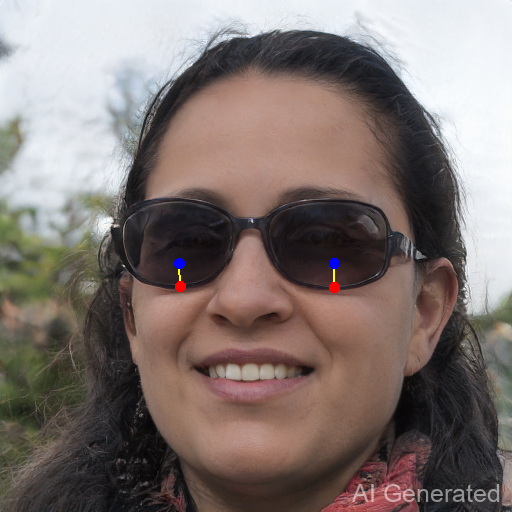
\includegraphics[width=\linewidth]{point_tracking/image_FFHQ/START.png}
    \caption*{初始状态}
\end{minipage}
\hfill
\begin{minipage}{0.6\linewidth}
    \centering
    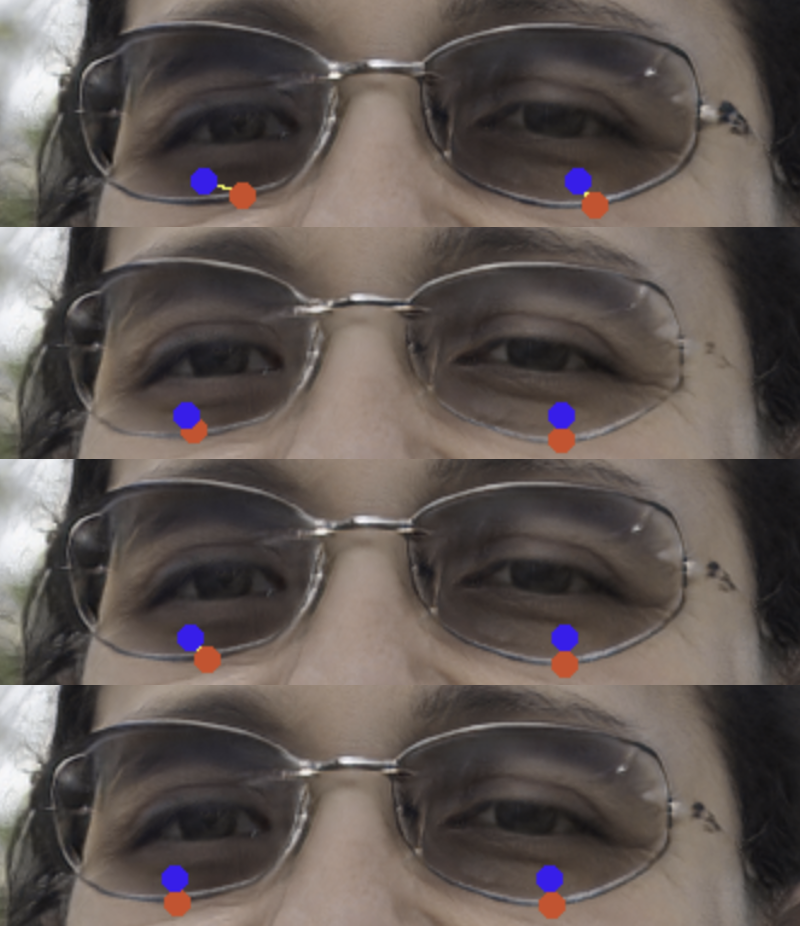
\includegraphics[width=\linewidth]{point_tracking/image_FFHQ/FFHQ.png}
    \caption*{四种方法对比}
\end{minipage}
\caption{FFHQ 墨镜编辑过程可视化（右图从上至下：NN, RAFT, HYBRID, MULTISCALE）}
\label{fig:ffhq}
\end{figure}

\subsubsection{实验二：FFHQ 额头编辑（弱纹理）}
本实验旨在评估追踪算法在弱纹理区域的表现。选取 FFHQ 样本，任务是将人脸额头部位的点向下拖拽，视觉效果表现为发际线向下移动。额头区域皮肤光滑，缺乏显著的角点或边缘特征，是典型的弱纹理场景。

实验数据（表 \ref{tab:weak}）呈现出明显的两极分化。\textbf{RAFT} (28.43 px) 的误差显著高于其他方法（约两倍），证实了在缺乏结构性纹理时，光流算法极易遭受"孔径问题"（Aperture Problem）困扰，即无法感知沿边缘方向的运动，导致严重的漂移或失效。

相比之下，\textbf{MULTISCALE} 提供了最佳的稳健性（13.24 px）。虽然其最终距离提升有限，但从定性的追踪过程观察来看，它避免了基线 NN 方法在迭代过程中出现的"跳跃"现象（即控制点在相邻的相似特征间不稳定切换）。通过利用多层特征的语义约束，MULTISCALE 实现了更加平滑稳健的追踪。

\begin{table}[H]
\centering
\small
\begin{tabular}{lcc}
\toprule
\textbf{方法} & \textbf{APD (px)} & \textbf{排名} \\
\midrule
MULTISCALE & \textbf{13.24} & 1 \\
NN & 13.48 & 2 \\
HYBRID & 13.66 & 3 \\
RAFT & 28.43 & 4 \\
\bottomrule
\end{tabular}
\caption{FFHQ 弱纹理编辑结果（$k=50$）}
\label{tab:weak}
\end{table}

\begin{figure}[H]
\centering
\begin{minipage}{0.25\linewidth}
    \centering
    
\includegraphics[width=\linewidth]{point_tracking/image_weak_texture/START.png}
    \caption*{初始状态}
\end{minipage}
\hfill
\begin{minipage}{0.6\linewidth}
    \centering
    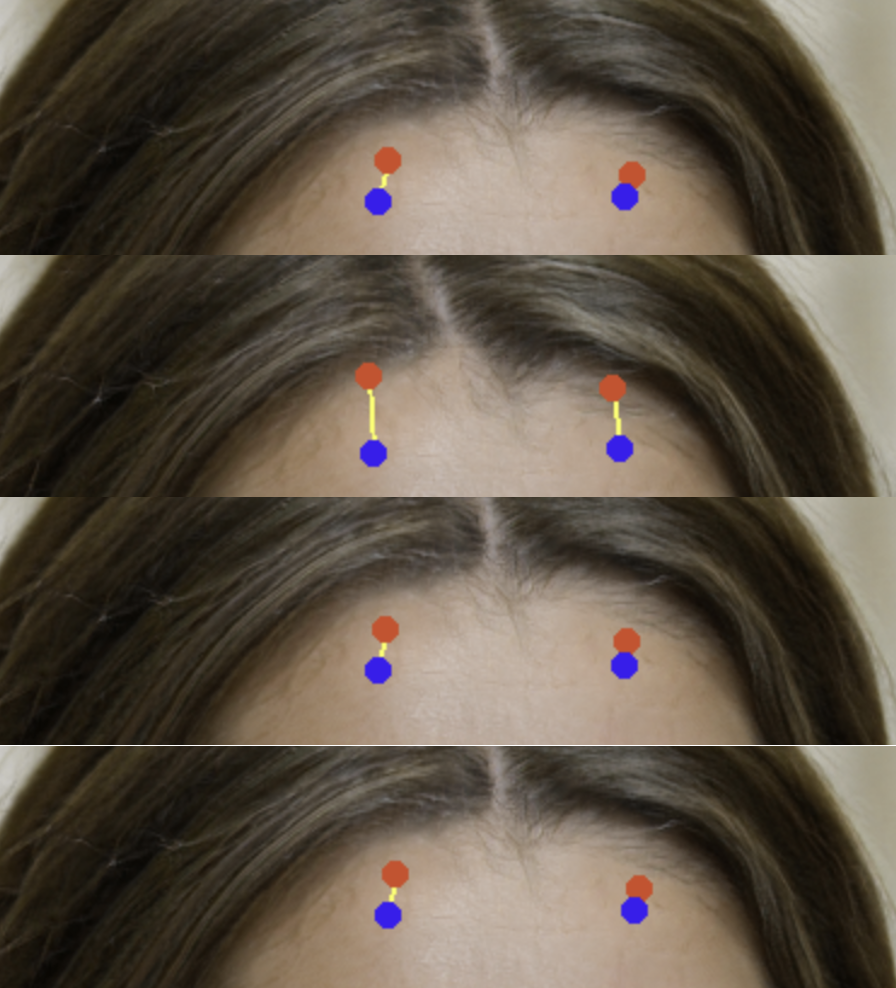
\includegraphics[width=\linewidth]{point_tracking/image_weak_texture/weak_texture.png}
    \caption*{四种方法对比}
\end{minipage}
\caption{弱纹理场景对比（右图从上至下：NN, RAFT, HYBRID, MULTISCALE）}
\label{fig:weak}
\end{figure}

\subsection{DragGAN vs DragDiffusion}

\subsubsection{领域内对比}
\textbf{人脸编辑：} 图 \ref{fig:human} 显示两者在嘴部编辑上表现相当。但在头发等弱纹理区域，DragDiffusion 表现更优，合成了自然的头发纹理；而 DragGAN 由于缺乏纹理线索，特征追踪失效，导致生成了杂乱的伪影。在鼻子编辑中，DragGAN 需 500 epoch 仍偏离目标，且身份发生漂移，而 DragDiffusion 200 epoch 即收敛，显示了其在处理大变形时的稳定性。

\begin{figure}[H]
\centering
\begin{subfigure}[b]{0.24\linewidth}
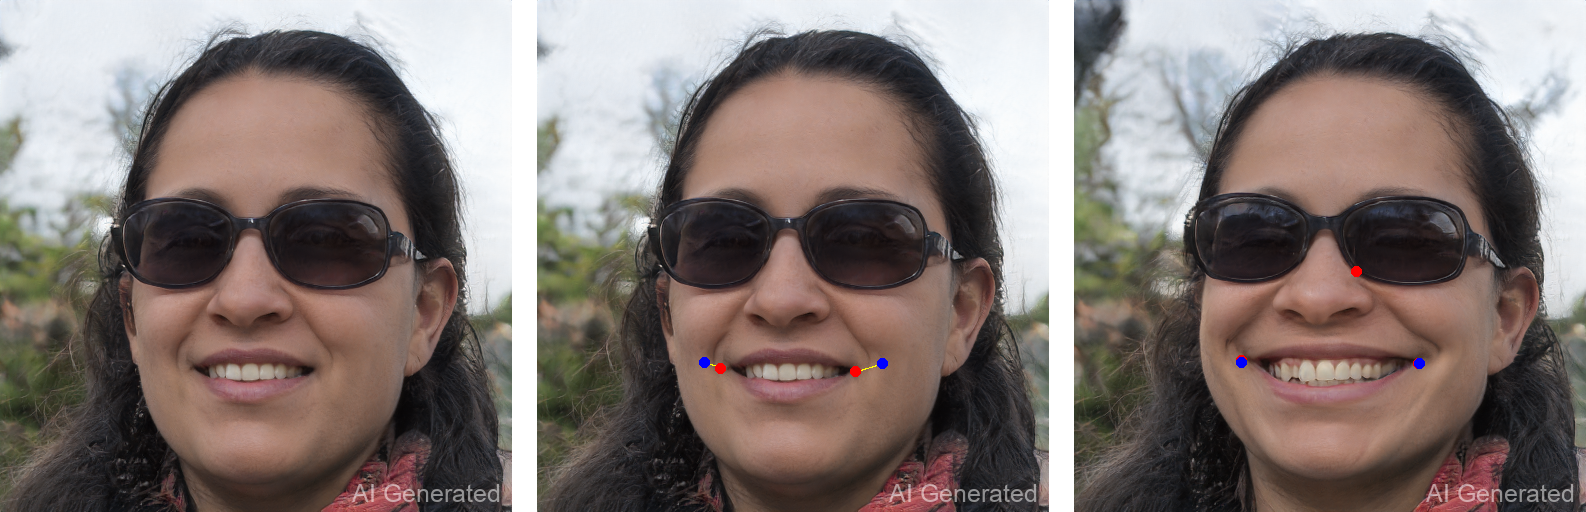
\includegraphics[width=\linewidth]{diff_comparison/_results_GAN/human_face/mouth.png}
\caption{GAN-嘴部}
\end{subfigure}
\begin{subfigure}[b]{0.24\linewidth}
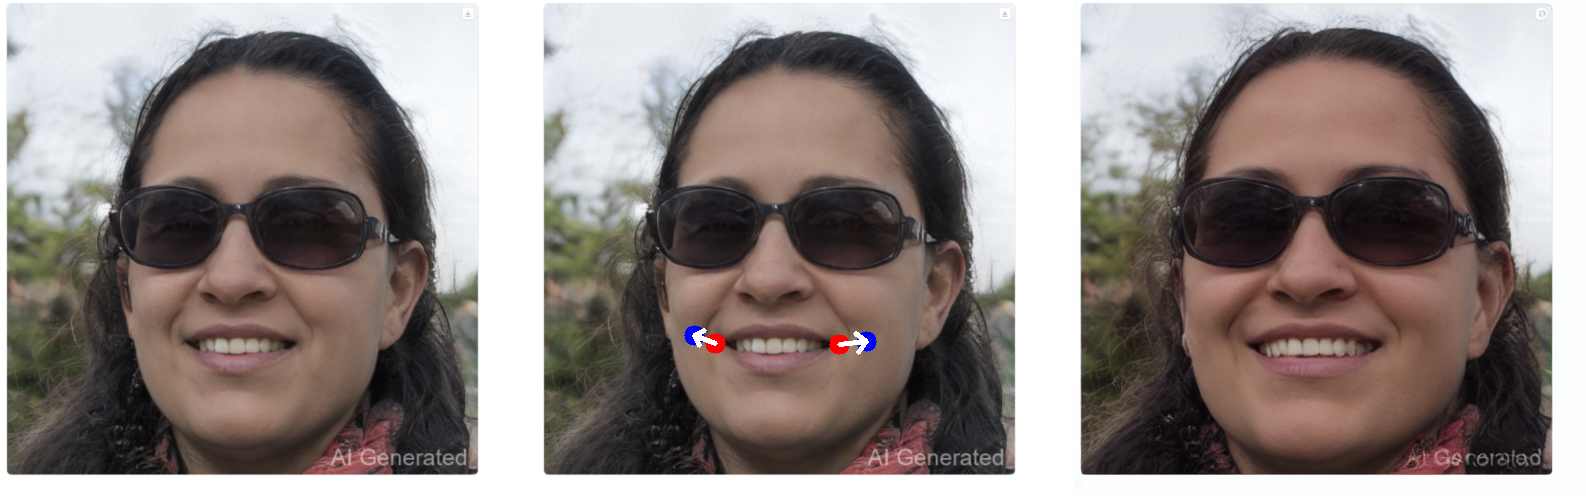
\includegraphics[width=\linewidth]{diff_comparison/_results_Diff/human_mouth.png}
\caption{Diff-嘴部}
\end{subfigure}
\begin{subfigure}[b]{0.24\linewidth}
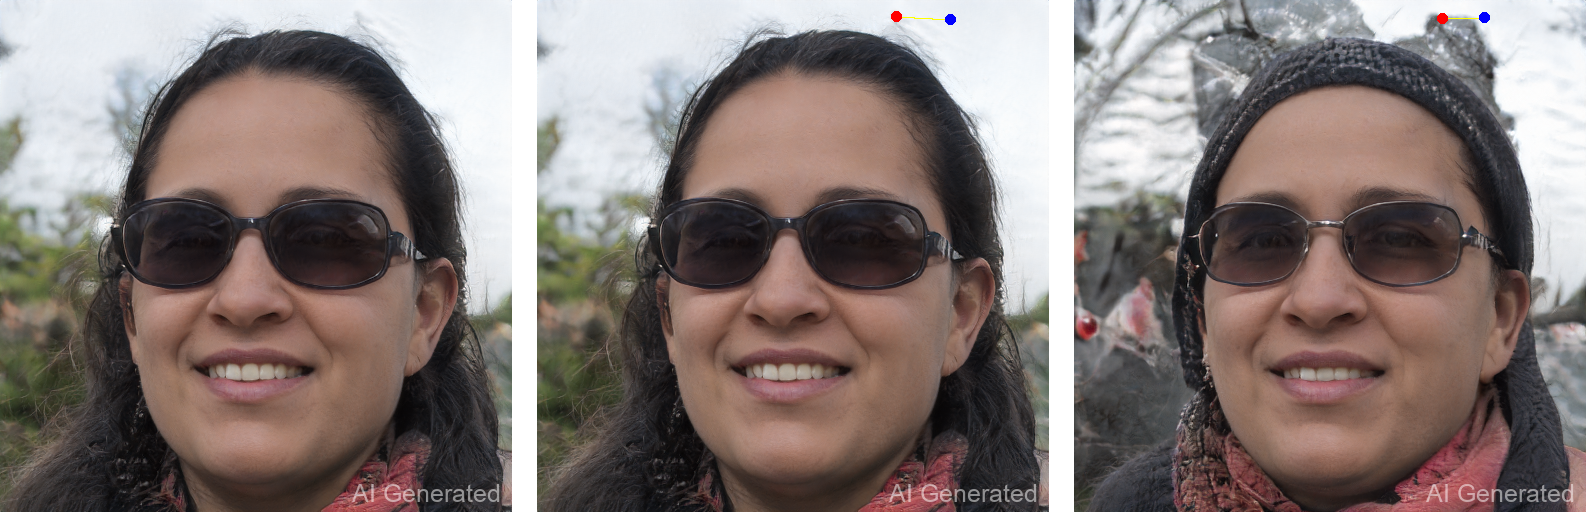
\includegraphics[width=\linewidth]{diff_comparison/_results_GAN/human_face/hair.png}
\caption{GAN-头发}
\end{subfigure}
\begin{subfigure}[b]{0.24\linewidth}
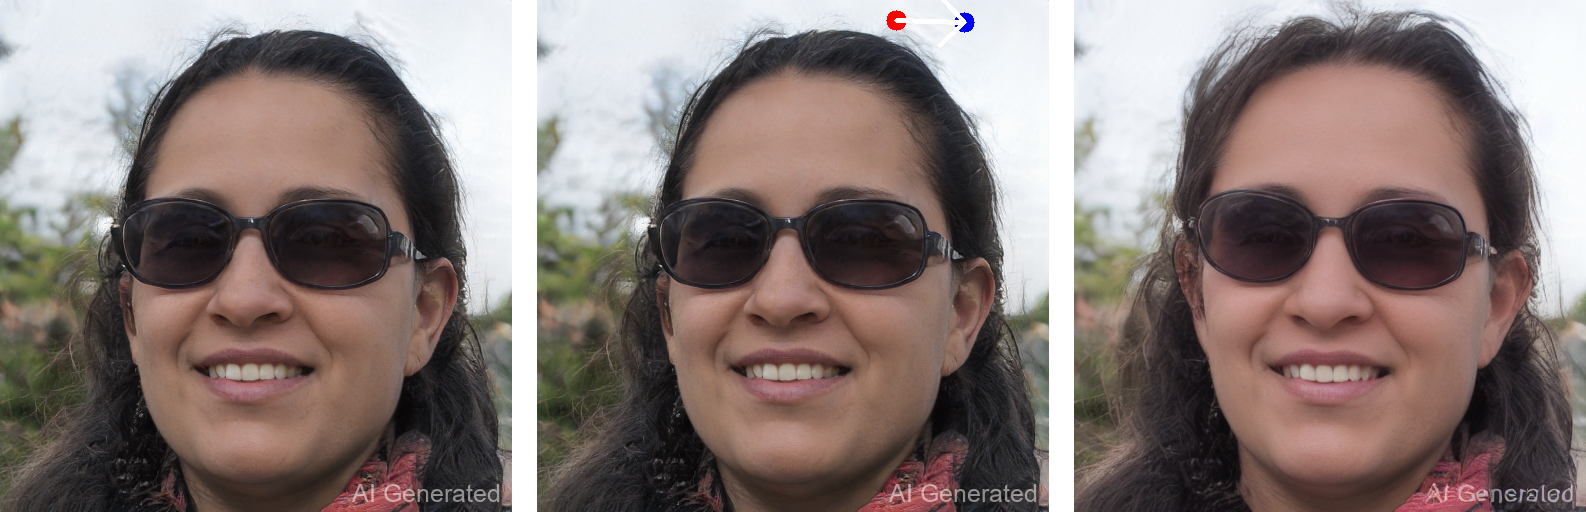
\includegraphics[width=\linewidth]{diff_comparison/_results_Diff/human_hair.png}
\caption{Diff-头发}
\end{subfigure}
\caption{人脸编辑对比}
\label{fig:human}
\end{figure}

\textbf{狮子编辑：} 图 \ref{fig:lion} 显示 DragGAN 在领域内对象上保持了完美的面部细节，而 DragDiffusion 导致严重扭曲。这表明虽然 Diffusion 模型具有通用性，但在特定细粒度结构（如动物五官）的保真度上，仍不如经过专门训练的 GAN 模型。

\begin{figure}[H]
\centering

\includegraphics[width=0.4\linewidth]{diff_comparison/_results_GAN/lion/nose.png}
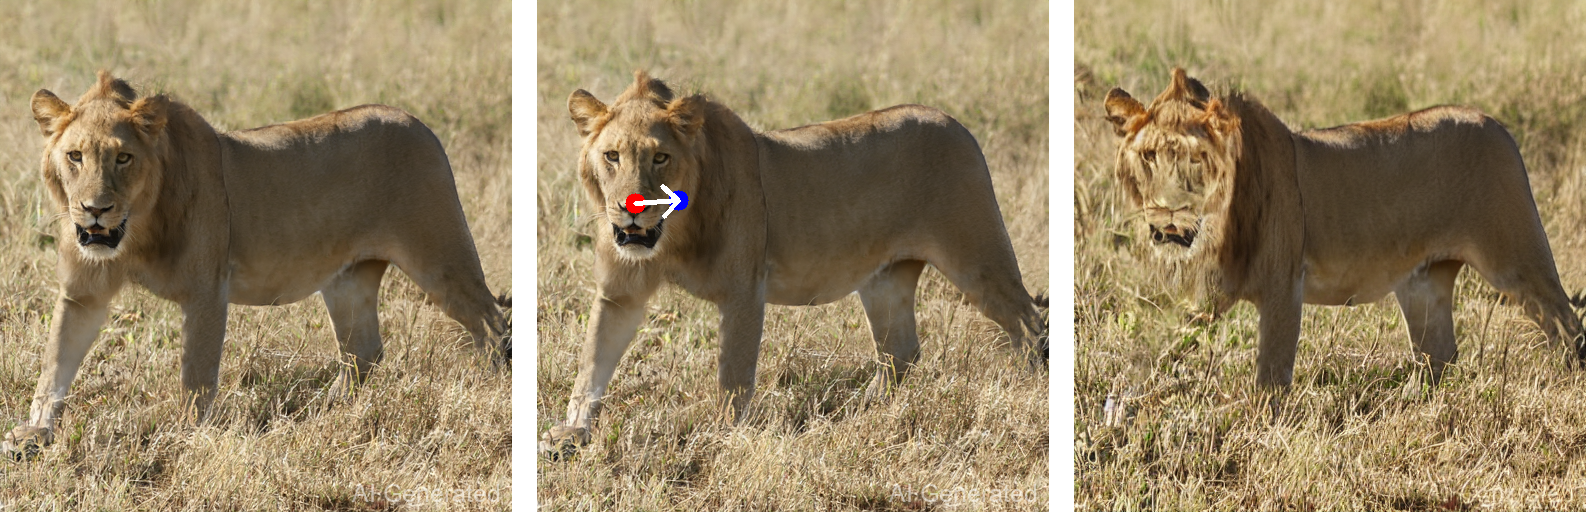
\includegraphics[width=0.4\linewidth]{diff_comparison/_results_Diff/lion_nose.png}
\caption{狮子编辑对比（左：DragGAN；右：DragDiffusion）}
\label{fig:lion}
\end{figure}

\subsubsection{开放域对比}
图 \ref{fig:open} 揭示了两种模型的本质差异。DragGAN 在山脉图像上完全失效，将场景扭曲为动物形状，这是因为 GAN 被限制在其训练数据的流形上（Manifold Constraint），无法生成流形外的图像。相反，DragDiffusion 利用 Stable Diffusion 庞大的先验知识，成功保持了山脉的地形结构。在艺术作品《星夜》上，DragDiffusion 同样有效处理了复杂背景，证明了其强大的通用性。

\begin{figure}[H]
\centering
\begin{minipage}{0.45\linewidth}
    \centering
    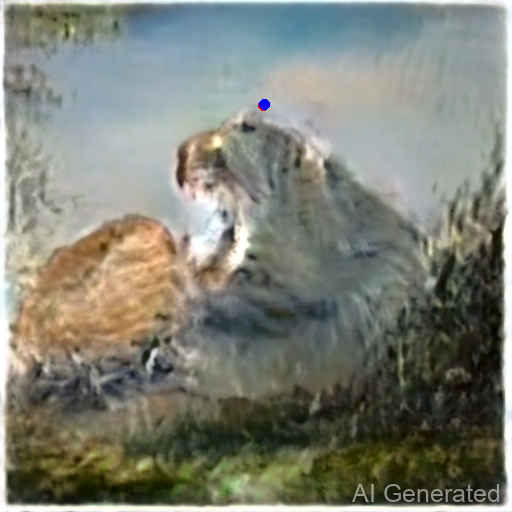
\includegraphics[width=\linewidth]{diff_comparison/_results_GAN/mountain/mountain_end.png}
    \caption*{(a) DragGAN-山脉}
\end{minipage}
\hfill
\begin{minipage}{0.45\linewidth}
    \centering
    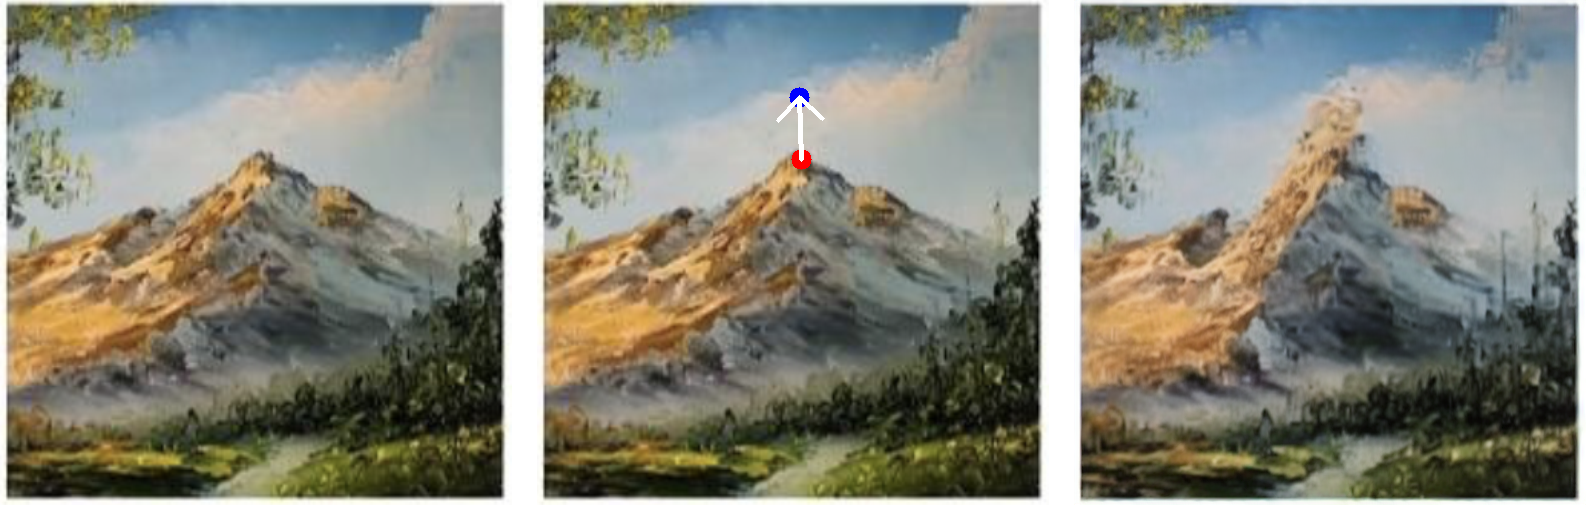
\includegraphics[width=\linewidth]{diff_comparison/_results_Diff/mountain_view.png}
    \caption*{(b) Diff-山脉}
    \vspace{0.5cm}
    
    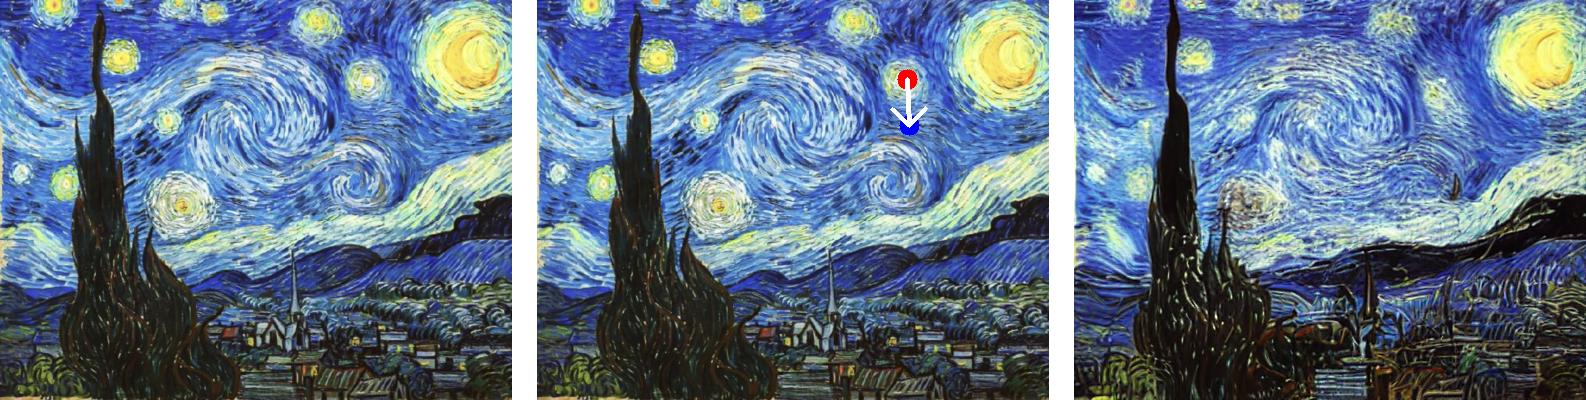
\includegraphics[width=\linewidth]{diff_comparison/_results_Diff/starry_night.png}
    \caption*{(c) Diff-星夜}
\end{minipage}
\caption{开放域编辑对比}
\label{fig:open}
\end{figure}

\section{结论}
本文提出的三项改进显著提升了 DragGAN 的实用性：(1) 特征融合机制有效抑制背景伪影，优于传统掩码损失；(2) 多尺度追踪在弱纹理场景下表现最稳健，建议作为默认策略；(3) 对比实验揭示了 DragGAN 在领域内精度优势与开放域泛化局限的权衡。未来工作可探索自适应追踪策略切换和基于文本引导的混合编辑框架。

\textbf{代码与数据：} 所有实验代码和补充材料已开源至 \url{https://github.com/CharlesChen397/DragGAN}。

\end{document}
